% Software Frontend (HTML/CSS/JS; Vue.js)
% Zuständig: Arthur

\section{Software - Frontend}
\label{sec:software_frontend}
Das Frontend ist eine Webseite und dient zur Visualisierung der gesammelten Daten vom Server.
Darunter zählen die Daten vom LiDAR-Sensor, vom Accelerometer und die Geschwindigkeit der Roboter
mithilfe der Encoder. Um das ganze geschehen der Roboter mitverfolgen zu können ohne hinterher rennen zu müssen
werden auch die Kamerabilder der unterschiedlichen Roboter angezeigt.

Das Frontend wird mithilfe von Vue.js programmiert. Vue.js ist ein JavaScript Framework und bietet 
verschiedene Möglichkeiten an die Webseite zu progammieren. Bei Vue.js kann man zwischen den Möglichkeiten "Options" und "Composition" unterscheiden.
Das Verhalten des Codes bleibt gleich, bietet aber eine andere Syntax. Der große Vorteil des Vue.js Frameworks ist, ist, dass es einem bietet 
HTML, CSS und JavaScript in eine sogenannte "SFC"\footnote{Single-File Components} einzubinden. Durch eine SFC schreibt man HTML, CSS und JavaScript in einer Datei, anstatt in vielen unterschiedlichen
die alle zueinander finden müssen.  

\subsection{LiDAR-Karte}
\label{subsec:frontend_lidar_map}
TODO neues Bild
\\
Die Ziel der LiDAR-Karte besteht darin auf dem User Interface bzw. der Webseite, die exakte
Position der Roboter anzuzeigen sowie die Wände, genauergesagt Hindernisse in der Umgebung. Hindernisse werden an Punkten auf der Karte festgestellt.

%wrapfigure Probleme beheben
%\begin{wrapfigure}{l}{0.5\textwidth}
%    \centering
%        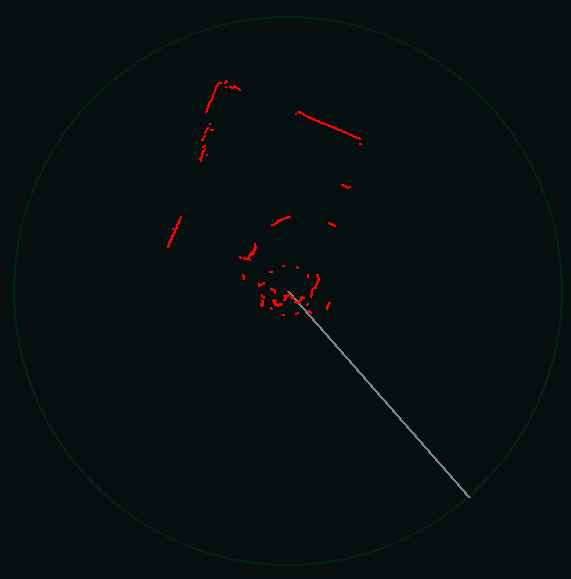
\includegraphics[width=0.5\textwidth]{img/LiDARMessung_alt.jpg}
%    \caption{LiDAR-Messung}
%    \label{fig:LiDAR-Messung}
%\end{wrapfigure}

\subsection{Fernüberwachung per Kamera}
\label{subsec:frontend_cam_stream}

\subsection{Fernsteuerung}
\label{subsec_frontend_control}

\subsection{Anzeigen der Sensordaten}
\label{subsec:frontend_sensors}